\documentclass[12pt,oneside,english]{report}
\usepackage[utf8]{inputenc}

\usepackage[a4paper,width=150mm,top=25mm,bottom=25mm]{geometry}
\usepackage[binary-units=true]{siunitx}
\usepackage[english=american]{csquotes}
\usepackage[hidelinks]{hyperref}
\usepackage[english]{babel}
\usepackage[style=iso-numeric,minnames=1,maxnames=3,giveninits,uniquename=init]{biblatex}
\usepackage[T1]{fontenc}
\usepackage[super]{nth}
\usepackage{amsmath}
\usepackage{array}
\usepackage{booktabs}
\usepackage{caption}
\usepackage{datetime}
\usepackage{fancyhdr}
\usepackage{float}
\usepackage{fontawesome5}
\usepackage{graphicx}
\usepackage{lipsum}
\usepackage{pgfplots}
\usepackage{subcaption}
\usepackage{tabularx}
\usepackage{tikz-qtree}
\usepackage{tikz}
\usepackage{tocbibind}

\addbibresource{references.bib}
\setlength{\bibhang}{0cm} % left-align bibliography
\setlength{\headheight}{15pt}

% textidote: ignore begin
\captionsetup{justification=centering}
% textidote: ignore end
\fancyfoot[C,C]{\thepage}
\fancyfoot{}
\fancyhead[R,L]{\leftmark}
\fancyhead{}
\renewcommand{\chaptermark}[1]{\markboth{\chaptername{} \ \thechapter.\ #1}{}}
\pagestyle{fancy}

\graphicspath{{images/}}

\sisetup{locale = US}

\usetikzlibrary{arrows.meta,calc,math,positioning,shadows,trees}
\tikzset{>=Stealth}
\pgfplotsset{width=9cm,compat=1.9}

\renewcommand*{\mkcitation}[1]{ #1}

\title{Passive Radar}
\date{December 2020}
\author{Andreas Baulig}

\begin{document}

% !TeX root = ./main.tex
% textidote: ignore begin
\begin{titlepage}
    \begin{center}
        \vspace*{1cm}
        \Huge
        \textbf{Passive Radar}

        \vspace{0.5cm}

        \LARGE
        Seminar Paper: Automotive Radar

        
\includegraphics[width=\textwidth]{hs-esslingen_logo.png}

        \large
        major \\
        \Large
        Computer Engineering (B.Eng.)

        \vspace{0.25cm}

        \large
        submitted by

        \vspace{0.25cm}

        \Large
        \begin{tabular}{c}
            \textbf{Andreas Baulig} \\
            matr.-nb.: 759720
        \end{tabular}

        \vspace{0.5cm}

        Faculty Information Technology \\
        at University of Esslingen

        \vfill

        \today

    \end{center}
\end{titlepage}
% textidote: ignore end

% !TeX root = ../main.tex
\begin{abstract}
\end{abstract}

% !TeX root = ../main.tex
% textidote: ignore begin
\chapter*{Ehrenwörtliche Erklärung}

Hiermit versichere ich, dass ich die vorliegende Ausarbeitung mit dem Titel \emph{Passive Radar} selbständig und ohne fremde Hilfe verfasst, und keine anderen als die angegebene Literatur und Hilfsmittel verwendet habe. Die Stellen der Arbeit, die dem Wortlaut oder dem Sinne nach anderen Werken entnommen wurden, sind in jedem Fall unter Angabe der Quelle kenntlich gemacht. Die Arbeit ist noch nicht veröffentlicht oder in anderer Form als Prüfungsleistung vorgelegt worden.

\vspace{4cm}

\begin{tabularx}{\textwidth}{ l X X}
    Andreas Baulig: & \hrulefill & \hrulefill   \\
    \vspace{1.5cm}  & Ort, Datum & Unterschrift \\
\end{tabularx}
% textidote: ignore end


\tableofcontents
\listoffigures

% !TeX root = ../main.tex
\chapter{Introduction}\label{chp:introduction}

Today's electromagnetic wave spectrum is sectioned into bands. While certain bands are inherently limited in their usefulness, due to atmospheric absorption, meteorologic, geologic or cosmic interference, most remaining bands are allocated to certain use-cases by regulatory institutions. The list of use-cases is immense and may range from radio astronomy, amateur radio, to maritime or aeronautical navigation, \emph{including radar}. However, possibly the largest holder of radio spectrum is \emph{telecommunications}. This reflects our societies growing demand for ever faster communications- and data-transfer-services. Sometimes this need conflicts or supersedes other use-cases. As with the recent 5G expansions in the L- and C-band, causing concerns for neighboring GPS~\cite{GPS.gov2020} and radar altimeter~\cite{RTCA2020} interest groups about their uninterrupted operability.

In the future, active radar system designers will likely have to fight for further spectrum-shares and defend against interference and displacements by a growing telecommunication interest. Whereas, passive radar systems, by nature, do not have to fight for their own spectrum. Contrary to active radar, passive radar can in fact piggyback off large telecom radio networks, and in a sense \textquote[{\cite[p.~1]{Malanowski2019}}]{recycle} ambient radiations from radio broadcasts and other types of emissions. Another benefit lies in passive radars inherent covertness, as such a system does not rely on emissions of its own. This on the other hand, makes passive radar heavily reliant on suitable illuminators in the vicinity.

\section{Definition}

As the term \emph{passive} implies, passive radar systems (also known as passive covert radar, passive coherent location or passive bistatic radar) do not emit their own radio energy in order to illuminate a target. Instead, they rely on other \emph{ambient} illuminators, which depending on type, may vary from conventional air surveillance radar, FM-radio, DAB, DVB-T, to Wi-Fi and Cellular~\cite[pp.~48--77]{Malanowski2019}\ \cite{Kuschel2013}. Due to the considerable spatial separation between sensor and illuminator passive radar is considered bistatic in nature. Figure~\ref{fig:topology} depicts the basic topology of a bistatic system, as employed by most passive radar systems. An illuminator sends out electromagnetic waves in the radio to microwave spectrum. These waves hit a target of interest, which will itself radiate a small portion of the received power back into the environment. The echo, as well as direct signal coming from the illuminator, arrive at the receiver with some delay and (in case the target is moving) Doppler frequency shift. Using intricate signal processing, a range and velocity is determined, details of which will be discussed in Chapter~\ref{chp:theory_of_operation}.

\begin{figure}
    \centering
    \begin{tikzpicture}
        \newcommand\drawTopology[4]{
    \coordinate (rx1_coord) at (-2,0);
    \coordinate (tx1_coord) at (2,0);
    \coordinate (target_coord) at (1.25,3);

    \node at (tx1_coord) [text width=0.5cm,text height=1cm] (tx) {};
    \node at (tx1_coord) [antenna,scale=0.5,below=-0.5cm] {};
    \path let \p1=(tx.north west), \p2=(tx.south east), \p3=(tx) in [label={below:Receiver}] ({\x3-0.4cm},\y1) rectangle ({\x3+0.4cm},\y2) node [below] at (\x3,\y2) {Illuminator};

    \node at (rx1_coord) [text width=0.5cm,text height=0.75cm] (rx) {};
    \node at (rx1_coord) [antenna,scale=0.5,below=-0.5cm] {};
    \path let \p1=(tx.north west), \p2=(tx.south east), \p3=(rx) in [label={below:Receiver}] ({\x3-0.4cm},\y1) rectangle ({\x3+0.4cm},\y2) node [below] at (\x3,\y2) {Receiver};

    \node at (target_coord) [label={above:Target}] (target) {\Huge\faPlane};

    \draw [visible on={#1},decorate,decoration={expanding waves,angle=35,segment length=4pt},blue!60] (tx) -- (target);
    \draw [visible on={#2},decorate,decoration={expanding waves,angle=25,segment length=4pt},red!60] (target) -- node [#4] {\small\contourlength{2pt}\contour{#3}{Echo}} (rx);
    \draw [visible on={#1},decorate,decoration={expanding waves,angle=15,segment length=4pt},blue!60] (tx) -- node [#4] {\small\contourlength{2pt}\contour{#3}{Reference}} (rx);
}

    \end{tikzpicture}
    \caption{Basic topology of a bistatic system.}\label{fig:topology}
\end{figure}

\section{History}

The first known system classifiable as passive radar dates back to Sir Robert Watson-Watt's \emph{Daventry Experiment} from 1935. It involved a \SI{10}{\kilo\watt} BBC radio transmitter, used as illuminator to detect a designated Heyford bomber~\cite[pp.~5--6]{Malanowski2019}~\cite{Kuschel2013}. Later, during the \nth{2} World War, Britain constructed the famous Chain Home radar network, which was an active radar system. A lesser known fact is that in 1942 the Germans built the Klein Heidelberg system. Following the passive radar approach, they detected incoming British aircraft, using their enemies Chain Home radar as illuminator. While the system demonstrated typical benefits associated with passive radar, i.e.\ resilience to certain forms of jamming, by means of chaff, its inception occurred too late as to have any deciding effect on the war~\cite{Griffiths2010}.

After WW2 focus shifted on active radar. Only around the 1980s interest was resurrected in the form of so called pulse chasing passive radar systems. These rely on emissions by  conventional active air surveillance radars and try to \emph{chase} along their pulses with an electronically steered antenna beam. Finally, by the 1990s work began on covert FM-radio based passive radar. This effort later expanded to support DAB and DVB-T emitters~\cite{Kuschel2013}. Their relatively high transmit power, in the order of few (DAB), several tens (DVB-T) to hundred \si{\kilo\watt} (FM)~\cite[p.~48, 57, 64]{Malanowski2019}, makes them comparable in power to active radar, when averaging pulse energy over pulse repetition interval.

% !TeX root = ../main.tex
\chapter{Theory of Operation}\label{chp:theory_of_operation}

Passive radar employs a wide variety of data processing techniques to accomplish target detection and measurement of both range and velocity relative to a sensing observer. It does so, by correlating target echos of ambient electromagnetic waves with the direct path reference signal originating from the illuminator. Doing so produces an ellipsoidal locus of possible bistatic target locations. Different methods are then used to solve the ambiguity of bistatic location and produce a probable cartesian position, relative to the sensor. In a strictly layered sense, this is where tracking and classification algorithms take over to definitely determine the object position and heading.

This chapter will follow the signal processing pipeline up to the point of cartesian location, by first introducing the fundamental principles inherent in bistatic systems. Next, methods of correlation are demonstrated, followed by mechanisms to solve the bistatic location ambiguity, and finally, transformation from the target location in bistatic to cartesian domain.

\section{Bistatic Geometry}

At the core of passive radar signal processing lies the concept of bistatic geometry. Figure~\ref{fig:bistatic_domain} depicts the topology of such a system. As illuminator and receiver exhibit considerable spatial separation (in the same order of magnitude as the sensor-target or illuminator-target separation)~\cite[p.~1571]{Griffiths2010}, special consideration of the resulting geometry is warranted. The following sections will introduce \emph{bistatic range} and \emph{bistatic velocity}.

\subsection{Bistatic Range}

Bistatic range \(R\) will be defined as the bistatic sum subtracted by the \emph{baseline} distance, shown in~\ref{equ:bistatic_range}.~\cite[p.~10]{Malanowski2019}

\begin{equation}\label{equ:bistatic_range}
    R=R_{1}+R_{2}-R_{\text{b}}
\end{equation}

With \(R_{1}\) representing the illuminator-target distance, \(R_{2}\) sensor-target distance, and \(R_{\text{b}}\) the direct line-of-sight distance or baseline distance between sensor (Rx) and illuminator (Tx). Figure~\ref{fig:bistatic_range} depicts a graphical perspective of the same equation.

\begin{figure}
    \centering
    \subcaptionbox{\label{fig:bistatic_domain}}[\textwidth]{
        \begin{tikzpicture}[x=1cm,y=1cm]
            % !TeX root = ../main.tex
\coordinate (rx1_coord) at (-2,0);
\coordinate (tx1_coord) at (2,0);
\coordinate (target_coord) at (1,1.25);

\node at (tx1_coord) [draw,fill=white] (tx1) {Tx};

\node at (rx1_coord) [draw,fill=white] (rx) {Rx};

\begin{scope}
    \clip
    let
    \p1=(target_coord),
    in
    (\x1 - 0.75cm,\y1 + 0.75cm) rectangle +(1.5,-1.5);
    \draw [color=gray]
    (2.42539052968,0) arc [start angle=0,end angle=360,x radius=2.42539052968,y radius=1.37204927807];
\end{scope}

\node at (target_coord) [label={[fill=white]above:Target}] (target) {\faPlane};

\draw [->,color=red] (tx1) -- node [black,midway,right,align=center] {$R_1$} (target);
\draw [->,color=red] (target) -- node [black,midway,left=4pt,align=center] {$R_2$} (rx);
\draw [->,color=blue] (tx1) -- node [black,midway,below,align=center] {$R_{\text{b}}$} (rx);

\pic [draw,angle radius=1cm,"$\beta$"] {angle=rx1_coord--target_coord--tx1_coord};

        \end{tikzpicture}
    }
    \subcaptionbox{\label{fig:bistatic_range}}[\textwidth]{
        \begin{tikzpicture}[x=1cm,y=1cm]
            % !TeX root = ../main.tex
\def\F{5}

\coordinate (rx1_coord) at (-\F,0);
\coordinate (tx1_coord) at (\F,0);
\coordinate (target_coord) at (3,3.5);

\draw [dotted,color=gray]
let
\p1=($(tx1_coord)-(target_coord)$),
\p2=($(target_coord)-(rx1_coord)$),
\p3=($(tx1_coord)-(rx1_coord)$),
\n1={veclen(\x1,\y1)},
\n2={\n1+veclen(\x2,\y2)},
\n3={\n2-veclen(\x3,\y3)}
in
(\n1,0) edge node [black,midway,right,align=center] {$+$} (\n1,-1)
(\n2,-1) edge node [black,midway,right,align=center] {$-$} (\n2,-2)
(\n3,-2) edge node [black,midway,right,align=center] {$=$} (\n3,-3);

\draw [->,color=red]
let
\p1=($(tx1_coord)-(target_coord)$),
\n1={veclen(\x1,\y1)}
in
(0,0) -- node [black,midway,above,align=center] {$R_1$} (\n1,0);
\draw [->,color=red]
let
\p1=($(tx1_coord)-(target_coord)$),
\p2=($(target_coord)-(rx1_coord)$),
\n1={veclen(\x1,\y1)},
\n2={\n1+veclen(\x2,\y2)}
in
(\n1,-1) -- node [black,midway,above,align=center] {$R_2$} (\n2,-1);
\draw [->,color=blue]
let
\p1=($(tx1_coord)-(target_coord)$),
\p2=($(target_coord)-(rx1_coord)$),
\p3=($(tx1_coord)-(rx1_coord)$),
\n1={veclen(\x1,\y1)},
\n2={\n1+veclen(\x2,\y2)},
\n3={\n2-veclen(\x3,\y3)}
in
(\n2,-2) -- node [black,midway,above,align=center] {$R_{\text{b}}$} (\n3,-2);

\draw [->,color=green]
let
\p1=($(tx1_coord)-(target_coord)$),
\p2=($(target_coord)-(rx1_coord)$),
\p3=($(tx1_coord)-(rx1_coord)$),
\n1={veclen(\x1,\y1)},
\n2={\n1+veclen(\x2,\y2)},
\n3={\n2-veclen(\x3,\y3)}
in
(0,-3) -- node [black,midway,above,align=center] {$R$} (\n3,-3);

        \end{tikzpicture}
    }
    \caption{Geometry of a bistatic system (\subref{fig:bistatic_domain}) and graphical representation of bistatic range (\subref{fig:bistatic_range}).}\label{fig:bistatic_geometry_and_range}
\end{figure}

The basis for determining bistatic range is measurement of time \(\tau\) the echo signal is delayed by, compared to the reference signal. In air and vacuum the signal speed can be reasonably approximated by the speed of light with \(c\approx\SI[per-mode=symbol]{3e8}{\metre\per\second}\). Thus bistatic range can be calculated as shown in~\ref{equ:bistatic_range_from_measurement}.~\cite[p.~11]{Malanowski2019}

\begin{equation}\label{equ:bistatic_range_from_measurement}
    R=c\cdot\tau
\end{equation}

Considering a constant bistatic sum \(R_{1} + R_{2}\) (see~\ref{equ:bistatic_range}), changing the terms of the sum \(R_{1}\) and \(R_{2}\) produces an ellipsoidal locus, with sender and receiver as foci. This so called \emph{bistatic ellipsoid} described by~\ref{equ:bistatic_ellipsoid} and graphed in figure~\ref{fig:bistatic_ellipsoid}, marks all possible target locations of equal bistatic range.

\begin{equation}\label{equ:bistatic_ellipsoid}
    \frac{x^2}{{\left(\frac{R_{1}+R_{2}}{2}\right)}^2} + \frac{y^2}{{\left(\frac{R_{1}+R_{2}}{2}\right)}^2 + \frac{R_{\text{b}}^2}{2}} + \frac{z^2}{{\left(\frac{R_{1}+R_{2}}{2}\right)}^2 + \frac{R_{\text{b}}^2}{2}} = 1
\end{equation}

\begin{figure}
    \centering
    \begin{tikzpicture}
        % !TeX root = ../main.tex
\def\R{25}
\def\F{10}
\def\a{sqrt((\R/2)^2)}
\def\b{sqrt((\R/2)^2 - \F^2)}
\def\c{\b}
\def\xmin{-int(\a + 5 - mod(\a - 5, 5))}
\def\ymin{-int(\b + 5 - mod(\b - 5, 5))}
\def\zmin{-int(\c + 5 - mod(\c - 5, 5))}
\def\xmax{+int(\a + 5 - mod(\a - 5, 5))}
\def\ymax{+int(\b + 5 - mod(\b - 5, 5))}
\def\zmax{+int(\c + 5 - mod(\c - 5, 5)))}
\begin{axis}[
        z buffer=sort,
        axis equal,
        colormap/viridis,
        samples=31,
        xmin=\xmin,
        ymin=\ymin,
        zmin=\zmin,
        xmax=\xmax,
        ymax=\ymax,
        zmax=\zmax,
        xlabel=$x$ \si{\kilo\metre},
        ylabel=$y$ \si{\kilo\metre},
        zlabel=$z$ \si{\kilo\metre},
        grid=major,
        view/az=25,
        view/el=30,
    ]
    \addplot3 coordinates {
            (\F,0,0)
            (\F,0,\zmin)
        } node[left,pos=0] {Rx};
    \addplot3 coordinates {
            (-\F,0,0)
            (-\F,0,\zmin)
        } node[left,pos=0] {Tx};
    \addplot3 [
        surf,
        shader=faceted interp,
        opacity=1,
        domain=0:180,
        y domain=0:360,
    ] (
    {\a*sin(x)*cos(y)},
    {\b*sin(x)*sin(y)},
    {\c*cos(x)}
    );
\end{axis}

    \end{tikzpicture}
    \caption{Bistatic ellipsoid for \(R=\SI{15}{\kilo\metre}\) and a baseline of \(R_{\text{b}}=\SI{10}{\kilo\metre}\). The points Tx and Rx mark the foci of the ellipsoid.}\label{fig:bistatic_ellipsoid}
\end{figure}

\subsection{Bistatic Velocity}

Appart from range, passive radar also offers ways of measuring target velocity. This measurement is based on doppler frequency shift of reference and echo signal. Due to the bistatic geometry however, this velocity is expressed as \emph{bistatic velocity}, and is defined in the most generic case, as rate of change of bistatic range. If it can be assumed that sender and receiver are stationary relative to each other, bistatic velocity \(V\) is defined as shown in~\ref{equ:bistatic_velocity}.~\cite[p.~12]{Malanowski2019}

\begin{equation}\label{equ:bistatic_velocity}
    V = -\lambda \cdot f_{\text{d}}
\end{equation}

With carrier wavelength given as \(\lambda=\frac{c}{f_{c}}\) and doppler frequency shift between reference and echo signals as \(f_{\text{d}}\).

Note that bistatic velocity and cartesian velocity are not linearly connected, as frequency shift depends on the radial speed towards (or away from) the sender \emph{and} receiver. To maintain a constant bistatic velocity the target has to travel co-linearly to the bisector of bistatic angle \(\beta/2\) (see Figure~\ref{fig:bistatic_domain}). Otherwise doppler shift, given by~\ref{equ:bistatic_doppler_shift}, depends on cartesian target velocity \(v\), angle between bistatic bisector and direction of velocity vector \(\delta\), and bistatic angle \(\beta\)~\cite[p.~39]{Griffiths2017}.

\begin{equation}\label{equ:bistatic_doppler_shift}
    f_{\text{d}} = \frac{2v}{\lambda} \cos{\left(\delta\right)}\cos{\left(\frac{\beta}{2}\right)}
\end{equation}

\section{Bistatic Range Equation}

Similarly to monostatic radar in which the \emph{radar equation} plays a major role, passive radar utilizes the bistatic range equation to capture many aspects of systems design. For a noise-less system with a isotropically reflecting target the received power \(P_{r}\) can be calculated as shown in~\ref{equ:bistatic_range_equation}.~\cite[p.~20]{Malanowski2019}

\begin{equation}\label{equ:bistatic_range_equation}
    P_{r} = \frac{P_{t} G_{t} \sigma G_{r} \lambda^2}{{\left(4 \pi \right)}^3 R_{1}^2 R_{2}^2}
\end{equation}

With \(P_{t}\) as transmit power (assuming isotropic radiation pattern); \(G_{t}\) and \(G_{r}\) describing the antenna gain of the transmitter and receiver antenna, target radar cross-section (RCS) \(\sigma\), the signal wavelength \(\lambda\), and the familiar sender-target and sensor-target ranges \(R_{1}\) and \(R_{1}\).

Compare this to the conventional radar equation for monostatic radar (\ref{equ:monostatic_radar_equation}), the only difference being the terms \(R_{1}^2 R_{2}^2\) (versus \(R^4\) for monostatic radar).~\cite[p.~4]{Kloeck2019}

\begin{equation}\label{equ:monostatic_radar_equation}
    P_{r} = \frac{P_{t} G_{t} \sigma G_{r} \lambda^2}{{\left(4 \pi \right)}^3 R^4}
\end{equation}

\section{Signal Correlation}

Determining the delay \(\tau\) between reference and echo signal is an essential step in solving the range equation. To extract this delay from the reference and echo radio signals, which are both continuous, a process called cross-correlated is used. This mathematical tool allows determining the displacement of two similar shaped time-shifted signals by effectively summing the products of two signals. Thus sections of low similarity are suppressed and sections of high similarity are amplified, resulting in peaks at the points of high similarity. Borrowing the approach also used in classic radar signal processing~\cite{Richards2014}, the cross-correlation of an echo signal \(x_e\) against a reference signal \(x_r\) in continuous domain is given by equation~\ref{equ:cross_correlation}.

\begin{equation}\label{equ:cross_correlation}
    \psi(t) = \int_{-\infty}^{\infty}{ x_{e}(\tau) x_{r}^{*}(\tau - t) \mathrm{d} \tau }
\end{equation}

Where \(*\) denotes the complex conjugation. While the integration limits here are defined as infinite, practical systems use a finite integration time or coherent processing interval, starting from several hundred milliseconds to several seconds.~\cite[p.~134]{Malanowski2019} This is one of the few variables the passive radar designer can actively control. Equation~\ref{equ:cross_correlation} can also be expressed in terms of bistatic range \(R\), as shown in equation~\ref{equ:cross_correlation_range}.

\begin{equation}\label{equ:cross_correlation_range}
    \psi(R) = \int_{-\infty}^{\infty}{ x_{e}(\tau) x_{r}^{*} \left( \tau - \frac{R}{c} \right) \mathrm{d} \tau }
\end{equation}

Figure~\ref{fig:signal_correlation} depicts the correlation of a simulated reference \(x_r\) and echo \(x_e\) signal. The echo signal is time shifted by \(\tau = \SI{600}{\micro\second}\) (corresponding to a bistatic range of \(R = \SI{180}{\kilo\metre}\), assuming a rate of propagation of \(c \approx 3 \cdot 10^{8}\)) and commingled with noise. Given by the equation \(P_n = BT\)~\cite[pp.~40--44]{Malanowski2019}, this noise is the result of a finite integration time \(T = \SI{1}{\milli\second}\) and an effective bandwidth of \(B = \SI{400}{\kilo\hertz}\). It can also be seen in the noise floor of Figure~\ref{fig:correlation_db}, which approximates the theoretical value of \SI{-26}{\deci\bel}. The correlation graphs~\ref{fig:correlation_db} and~\ref{fig:correlation_linear} both show a clear peak in similarity at around \SI{600}{\micro\second}, which matches the expectation given the input.

\begin{figure}[h]
    \centering
    \subcaptionbox{\label{fig:reference_signal}}{
        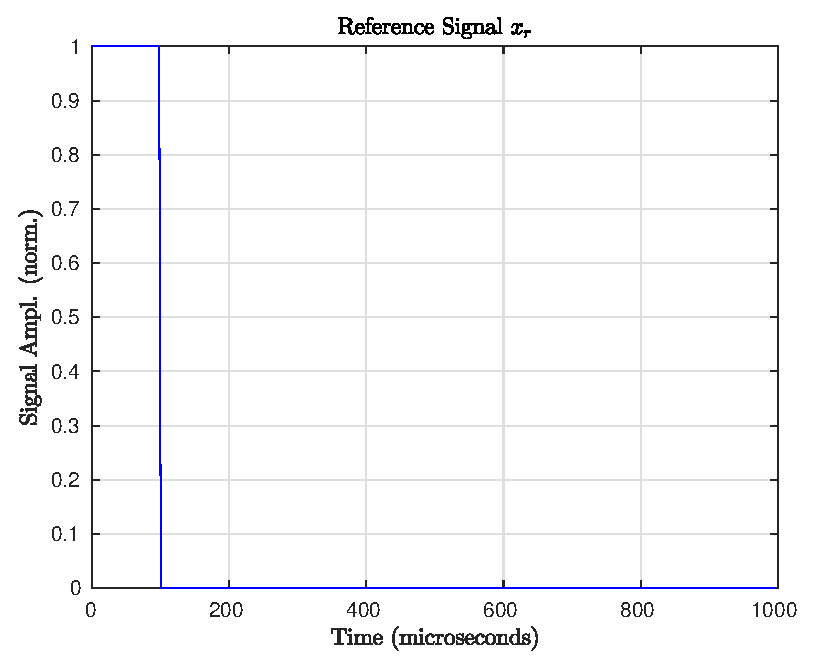
\includegraphics[width=0.47\textwidth]{reference_signal.eps}
    }
    \subcaptionbox{\label{fig:echo_signal}}{
        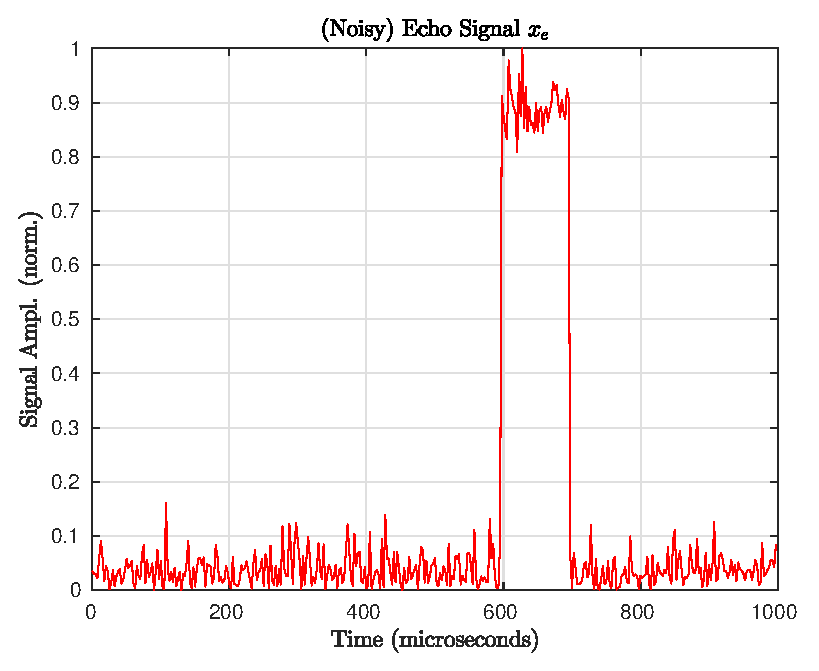
\includegraphics[width=0.47\textwidth]{echo_signal.eps}
    }
    \linebreak
    \subcaptionbox{\label{fig:correlation_db}}{
        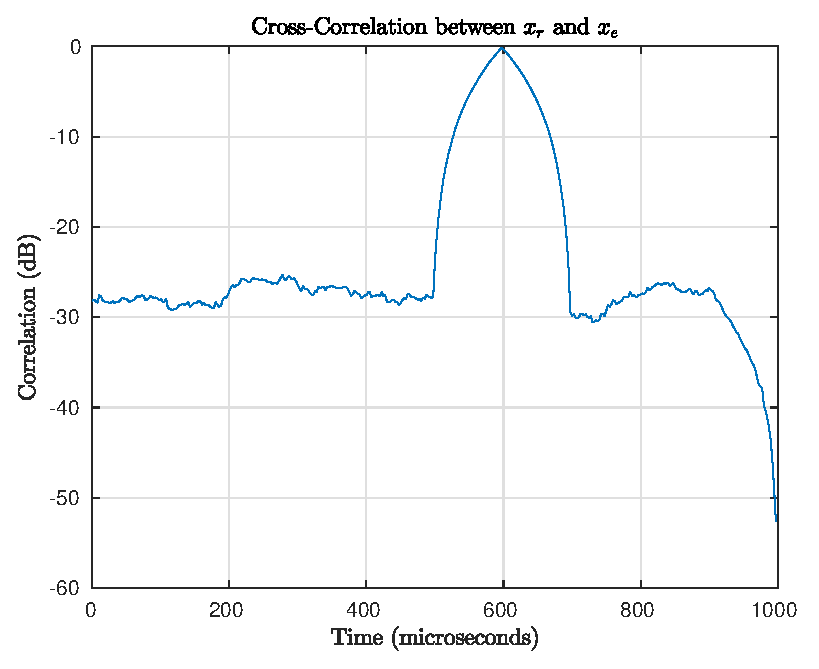
\includegraphics[width=0.47\textwidth]{correlation_db.eps}
    }
    \subcaptionbox{\label{fig:correlation_linear}}{
        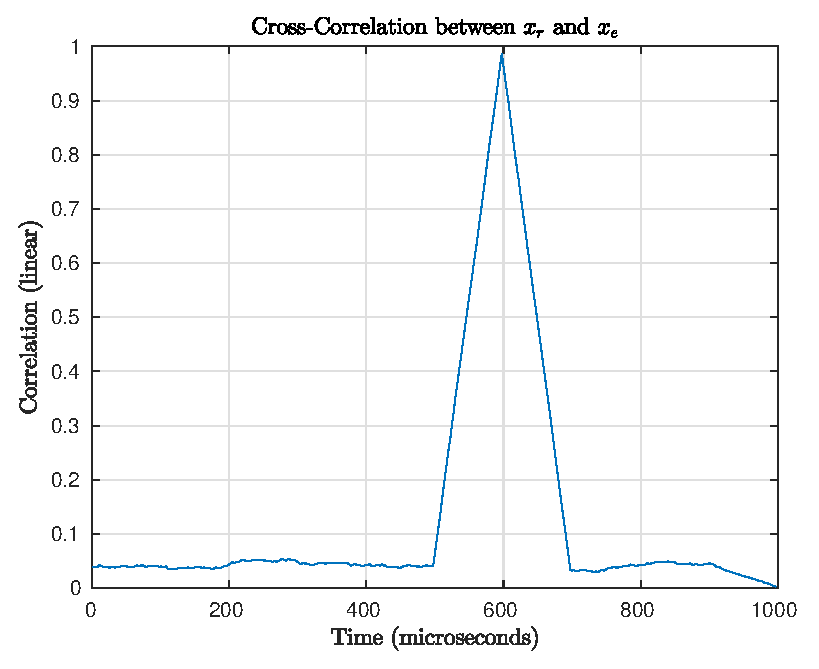
\includegraphics[width=0.47\textwidth]{correlation_linear.eps}
    }
    \caption{Correlation of reference signal (\subref{fig:reference_signal}) and echo signal (\subref{fig:echo_signal}), in both \si{\deci\bel} (\subref{fig:correlation_db}) and linear scale (\subref{fig:correlation_linear}).}\label{fig:signal_correlation}
\end{figure}

While cross-correlation can already be used to determine the time shift \(\tau\) and thus bistatic range, doppler shift of the signal provides information on the target bistatic velocity. It is possible to extend the cross-correlation equation, shown in~\ref{equ:cross_correlation}, by a second dependant variable, representing doppler shift. This leads to the cross-\emph{ambiguity} function (CAF), as shown in equation~\ref{equ:cross_ambiguity_function}.

\begin{equation}\label{equ:cross_ambiguity_function}
    \psi(\tau, f_{d}) = \int_{-T/2}^{T/2} {x_{e}(t) \cdot x_{r}^{*}} \left( t - \tau \right)\mathrm{e}^{\mathrm{j} 2 \pi f_{d} t} \mathrm{d} t
\end{equation}

Note that this equation already incorporates a finite coherent processing interval \(T\). As modern passive radar systems usually operate in the digital domain, it makes sense to express the CAF in terms of discrete samples. Using \(T = N / f_{s}\) as substitution for CPI, where \(N\) denotes the number of samples captured per interval; and \(f_{s}\) expressing the sampling frequency, this leads to equation~\ref{equ:cross_ambiguity_function_digital}~\cite[p.~134]{Malanowski2019}.

\begin{equation}\label{equ:cross_ambiguity_function_digital}
    \psi(m,k) = \sum_{n = 0}^{N - 1}{x_{e}(n) \cdot x_{r}^{*}(n - m) \mathrm{e}^{-\mathrm{j} \frac{2 \pi}{N} k n}}
\end{equation}

Here, bistatic velocity is expressed in terms of an integer number of sample delays \(m\). Similarly, bistatic velocity is measured in terms of an integer number of frequency bins \(k\), that the two signals are separated by doppler shift.

This concludes the necessary theoretical foundations to determine bistatic range and velocity. Practical systems employ different methods to efficiently implement these ideas in digital signal processors. One of which, described by~\cite[p.~138]{Malanowski2019}, bears striking similarities to conventional active radar matched filtering and doppler processing. This method is generally referred to as \emph{the batch algorithm}. It's core principle is presented in derivation~\ref{equ:batch_algorithm}.

\begin{equation}\label{equ:batch_algorithm}
    \begin{split}
        \psi(m,k) & = \sum_{q = 0}^{Q - 1}{\sum_{p = 0}^{P - 1}{x_{e}(q P + p) x_{r}^{*}(q P + p - m) \mathrm{e}^{-\mathrm{j} \frac{2 \pi}{N} k (q P + p)}}} \\
        & \approx \sum_{q = 0}^{Q - 1}{ \left\{ \sum_{p = 0}^{P - 1}{ \left\{ x_{e}(q P + p) x_{r}^{*}(q P + p - m) \right\} } \mathrm{e}^{-\mathrm{j} \frac{2 \pi}{N} k q} \right\} } \\
        & \approx \operatorname{FFT} \left\{ \sum_{p = 0}^{P - 1}{ x_{e}(q P + p) x_{r}^{*}(q P + p - m) } \right\} \\
        \\
        & \approx \operatorname{FFT} { \left\{ \operatorname{COR} { \left\{ x_{e}(q P + p), x_{r}^{*}(q P + p) \right\} } \right\} }
    \end{split}
\end{equation}

Here, samples are \emph{batched} into \(Q\) number of blocks; the \emph{slow time} domain. The number of samples per block is given by \(P\). Within a block the term \emph{fast time} is used. It is assumed within fast time, doppler shift is negligible, allowing the phase shift term to be simplified, and dragged outside the inner sum over \(P - 1\). This happens in line two of~\ref{equ:batch_algorithm}. Realizing that \(\sum_{n = 0}^{N - 1}{ x_{n} \mathrm{e}^{-\mathrm{j} \frac{2 \pi}{N} k n} } \equiv \operatorname{FFT}{ \left\{ \right\} }, k = 0, \dots, N - 1 \), the outer sum can be substituted by a fast fourier transformation (\(\operatorname{FFT}\)). This leads to the expression in line three of~\ref{equ:batch_algorithm}. Finally the inner sum over \(P - 1\) is expressed using the cross-correlation operator \(\operatorname{COR}\).


\printbibliography

\end{document}
